\documentclass[a4paper, norsk, 11pt]{article}
\usepackage[T1]{fontenc} 			% N�dvendig for fonter
\usepackage[latin1]{inputenc} % N�dvendig for ���
\usepackage{babel}						% N�dvendig for dokument
\usepackage{graphicx}					% For � kunne inkludere grafikk
\usepackage{amsmath, amsfonts, amssymb} % Pakker for � skrive matte
\usepackage[amssymb]{SIunits} % For � bruke \unit til SI-enheter
\usepackage{float} % For � bruke H som posisjon

% Tegninger, som b�ndgap
\usepackage{tikz,tkz-tab}
\usetikzlibrary{decorations.pathmorphing}
\usetikzlibrary{decorations.pathreplacing} % For � bruke kr�llparantes (brace)
\usetikzlibrary{shapes,arrows}
\usepackage{xcolor} % Farger
\usepackage{rotating} % Rotere p� stash

\usepackage[bookmarks]{hyperref} % For linker til kapitler
\usepackage{url}

\author{Jon Skarpeteig}
\title{Basis dokument}
\date{\today}


\begin{document}
 \DeclareGraphicsExtensions{.pdf,.jpg,.png}
	\graphicspath{{./bilder/}}
\maketitle

%\section{Introduksjon}

%%INCOMPLETE - mangler masse + stash er feil

Solceller er antatt � dominere energisektoren de neste hundre �r. For at dette skal bli tilfelle trengs det billige og effektive solceller. Multikrystallinsk silisium er materialet som har mest potensiale for � oppn� dette. Det er billig � produsere, men har ogs� relativt lav utnyttelse av solenergien. Derfor er det viktig � n�yaktig kunne identifisere kilder til tap, og forst� virkem�ten til slike materialer. 

Det er oppdrettet et laboratorium for � kunne gj�re m�linger p� slike celler ved hjelp av fotoluminisens p� ekstremt lave temperaturer. Tidligere m�linger av multikrystallinsk silisium p� dette laboratoriet viser deler av et spekter som er � finne p� tilsvarende m�linger (f.eks \cite{tarasov00}), men deler av tapsspekteret som var forventet dukket ikke opp. Dette prosjektet fokuserer p� hva som er �rsaken til dette avviket, og hvordan det kan utbedres. I tillegg til det er det fokusert p� virkem�te til solceller, og kilder til tap i multikrystallinsk silisium.
\section{Solcelle teori}

%TEORIDEL - Solceller - virkem�te, karakteristikker, MC vs. Thinfilm, utforming, 

De fleste solceller er krystallinske, det betyr at strukturen er ordnet, eller periodisk. I praksis vil krystallene inneholde feil av forskjellige slag. Noen solcellematerialer er ikke krystallinske, men mangler langtrekkende periodisitet. Disse best�r da av amorfe materialer.

Et fritt elektron i vakuum vil kunne innta en hvilken som helst energi. Et elektron i en krystallstruktur er bundet av energib�nd atskilt av gap med energitilstander som elektronene ikke kan ha. Det er derfor bare plass til et endelig antall elektroner i hvert b�nd, fordi hver tilstand bare kan romme to elektroner i f�lge Pauli-Prinsippet. For en krystall kan energib�ndene oppfattes som overlapp av enkelttilstander for hvert atom. En kan oppfatte energib�ndene som krystallens 'elektronskall'. 

\begin{figure}[!h]
 \centering
 	% Tegning
 	\begin{tikzpicture}[scale=0.5]
     	\draw[very thick,->] (1,6) -- node[below] {x}  (25,6); % X akse
    	\draw[very thick,->] (1,6) -- node[left] {\begin{sideways}Energi\end{sideways}} (1,18); % Y akse
    
    \begin{scope} % Valens og ledningsb�nd
		    \draw[thick,fill=black!10] (2,7) rectangle node {Valensb�nd} ++(22,4);
        \draw[thick,fill=black!10] (2,13) rectangle node {Ledningsb�nd} ++(22,4);
        \draw[thick,<->] (13,13) -- node[right] {B�ndgap} (13,11); % Pil
    \end{scope}
    \end{tikzpicture}    \caption{Energib�nd}
    \label{fig:energiband}
\end{figure}

Det �verste b�ndet kalles ledningsb�ndet. Energib�ndet umiddelbart under ledningsb�ndet, kalles valensb�ndet. De ikke tillatte tilstandene mellom valensb�ndet og ledningsb�ndet kalles b�ndgapet. Dette b�ndgapet er veldig viktig i forbindelse med solceller og oppgis ofte i elektronvolt (eV). % Legg til kr�llstash p� figur

For at elektronet skal kunne flytte p� seg m� det befinne seg i ledningsb�ndet. Et elektron m� ha nok energi til � kunne eksiteres fra valensb�ndet. Eksitasjon vil si at et elektron forflytter seg fra valensb�ndet til ledningsb�ndet. Dette kan skje ved at elektronet f�r h�y nok energi til � forflytte seg over b�ndgapet ved termisk energi, eller annen energi tilf�rt utenfra, som fra lys. Dette gir �kt ledningsevne til materialet. Samtidig blir det en ledig plass i valensb�ndet, som gj�r at andre elektroner i valsensb�ndet kan f� h�yere kinetisk energi p� grunn av f�rre kollisjoner. Dette p�virker ogs� materialet slik at det f�r h�yere ledningsevne.

Materialer deles ofte inn i tre kategorier; Isolatorer, halvledere, og metaller. Isolatorer har ingen, eller f� elektroner i ledningsb�ndet, som gir dem d�rlig ledningsevne. Metaller har som regel fylte ledningsb�nd ved romtemperatur, som gir dem god ledningsevne. Selv ved 0K har metaller et delvis fylt ledningsb�nd. Halvledere har d�rligere ledningsevne enn metaller, og vil ved 0K ikke ha noen elektroner i ledningsb�ndet. B�ndgapet til halvledere ligger mellom det for isolatorer og metaller, slik at ved romtemperatur er ledningsb�ndet delvis fylt, i motsetning til isolatorer.

\begin{figure}[!h]
 \centering
 % Tegning
 

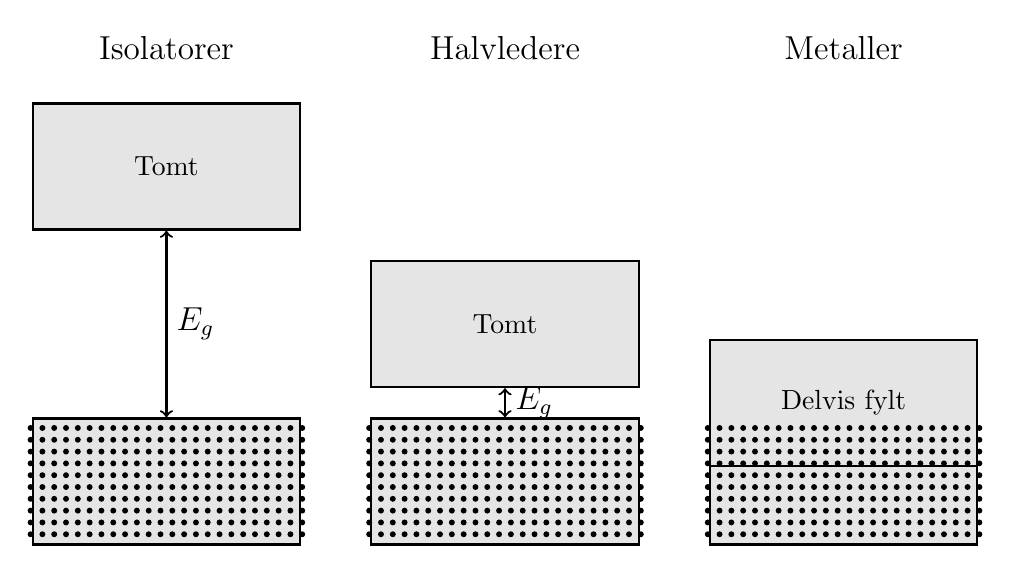
\begin{tikzpicture}
 	% Styles til elementer (kan ogs� v�re generelle utenfor tikzpicture)
	\tikzstyle{ledningsband} 	=	[rectangle, draw, thick, fill=black!10, text width=9em, text centered, minimum height=1.6cm]
	\tikzstyle{valensband}		= [rectangle, draw, thick, fill=black!10, text width=9em, text centered, minimum height=1.6cm]


	% Boksene i bunnen
	\node[valensband]	(valens_isolator)																										{};
	\node[valensband]	(valens_halvleder)	[right of=valens_isolator,  node distance=4.3cm]	{};
	\node[valensband]	(valens_metall)			[right of=valens_halvleder, node distance=4.3cm]	{};	
	
	% Boksene i toppen
	\node[ledningsband]	(lednings_isolator)		[above of=valens_isolator, 	node distance=4cm]	{Tomt};
	\node[ledningsband]	(lednings_halvleder)	[above of=valens_halvleder, node distance=2cm]	{Tomt};
	\node[ledningsband]	(lednings_metall)			[above of=valens_metall, 		node distance=1cm]	{Delvis fylt};
	
	% Piler
	\draw[thick,<->] (valens_isolator)  -- node[right] {\large $E_g$} (lednings_isolator);
	\draw[thick,<->] (valens_halvleder) -- node[right] {\large $E_g$} (lednings_halvleder);
	
	% Tekst p� toppen
	\node (isolator_tekst)  [above of=lednings_isolator,node distance=1.5cm]	{\large Isolatorer};
	\node (halvleder_tekst) [right of=isolator_tekst, 	node distance=4.3cm] 		{\large Halvledere};
	\node (metaller_tekst)  [right of=halvleder_tekst, 	node distance=4.3cm] 		{\large Metaller};
	
	% Elektroner i valensb�nd
	\foreach \y in {0,0.15,...,1.4}
		\foreach \x in {0,0.15,...,3.5} {
			\draw (\x-1.725,\y-0.67) circle (0.03cm) [fill=black];	% Isolator
			\draw (\x+2.575,\y-0.67) circle (0.03cm) [fill=black];	% Halvleder
			\draw (\x+6.875,\y-0.67) circle (0.03cm) [fill=black];	% Metall
		}	
	
\end{tikzpicture}

	    \caption{Typiske b�ndgap ved 0K} 
 \label{fig:bandgap}
\end{figure}
\vspace{30mm}

Typisk b�ndgap for halvleder silisium er 1.1eV, sammenlignet med 5eV for diamant som er en isolator. ~\cite[Kapittel 3]{streetman}

Hull er en beskrivelse for frav�r av elektroner i valensb�ndet. Et hull vil oppst� n�r et elektron eksiteres fra valensb�ndet til ledningsb�ndet. Lite b�ndgap, og h�y temperatur vil gi vesentlig flere elektroner i ledningsb�ndet, enn for lave temperaturer og stort b�ndgap. Dette beskrives med massevirkningsloven:

\begin{equation}
np=N_cN_ve^{-\frac{E_g}{kT}}
\label{eq:massevirkningsloven}
\end{equation}

der $n$ er antall elektroner, $p$ er antall hull, $N_c$ og $N_v$ er konstanter for gitte materialer. $E_g$ er b�ndgapet, $k$ er Boltzmanns konstant og $T$ er temperaturen i Kelvin. For en intrinsikk halvleder, det vil si en halvleder uten noe form for doping, for eksempel ren silisium, kan massevirkningsloven skrives:

\begin{equation}
np=n_i^2
\label{eq:massevirkningsloven_intrinsikk}
\end{equation}

der 

\begin{equation}
n_i=\sqrt{N_c N_v}e^{-\frac{E_g}{2kT}}
\label{eq:intrinsikk}
\end{equation}

Fra massevirkningsloven kommer det av $E_g$ er en avgj�rende faktor for om en krystall kan sies � v�re en halvleder eller ikke. 


\subsection{Doping}

Ved � sette inn andre atomer i en krystallstruktur, med en annerledes elektronfordeling er det mulig � �ke elektroner i ledningsb�ndet uten � endre konsentrasjonen av hull i valensb�ndet. Dette kalles donor-doping. Et eksempel p� donor-doping er � tilsette fosfor i en silisiumkrystall. Dette vil f�re til flere elektroner i ledningsb�ndet, da fosfor har et valenselektron mer enn silisium og valensb�ndet er tiln�rmet fullt. Fosfor vil i dette tilfellet kalles donor i denne donor-dopingen. Doping konsentrasjonen er vanligvis s� liten at b�ndstrukturen ikke forstyrres vesentlig. Hvis en for eksempel setter inn bor istedenfor fosfor, vil silisium krystallen bli akseptor-dopet. Bor har et mindre elektron i valensb�ndet enn silisium, og vil derfor tilf�re et hull ekstra i valensb�ndet. Som regel er donorkonsentrasjonen av hull og elektroner i henholdsvis valens- og ledningsb�nd vesentlig h�yere enn den intrinsikke, slik at det er en god tiln�rming � sette

\begin{equation}
n \approx N_d
\label{eq:donordoping}
\end{equation}

for donordoping, og

\begin{equation}
n \approx N_a
\label{eq:akseptordoping}
\end{equation}

for akspetordoping. Der $N_d$ er donorkonsentrasjonen, og $N_a$ er akseptorkonsentrasjonen.

En dopet halvleder omtales generelt som ekstrinsikk. Hvis en halvleder er dopet med overtall av donor atomer, har den overtall av elektroner, og kalles n-dopet. For akseptordoping omtales halvlederen som p-dopet, da den har overtall av hull. Den dominerende ladningsb�rertypen kalles for majoritetsb�reren. Majoritetsb�rerene vil v�re de som i hovedsak s�rger for str�mtransporten gjennom halvlederen.


\subsection{Transport- og rekombinasjons-prosesser}

Det er to mekanismer som bidrar til transport av elektroner og hull i halvledere: drift og diffusjon. Drift er transport av en ladd partikkel p� grunn av et elektrisk felt. For transport av et hull i en dimensjon er str�mmen $I_p$ lik antall hull $N_p$ ganger ladning $q$ som krysser et tverrsnitt.

\begin{equation}
I_p = N_p q
\label{eq:diffusjonsstrom}
\end{equation}

I vakuum vil et elektrisk felt akselerere hullene, og hastigheten vil stadig �ke. I halvledere vil det oppst� kollisjoner med atomene i halvlederen, som gir hullene en midlere hastighet s� lenge feltet er konstant. Denne midlere driftshastigheten er relatert til feltet via hullenes mobilitet $�_p$

\begin{equation}
v_p = �_p E
\label{eq:elektronfart}
\end{equation}

Hvis alle hullene beveger seg i samme retning kan en da beregne str�m per areal, eller str�mtetthet.

\begin{equation}
J_p = \frac{I_p}{A} = \frac{N_p q}{A} = pAv_p \frac{q}{A} = pv_p q = pq�_p E
\label{eq:hulltetthet}
\end{equation}

Kombinert med tilsvarende uttrykk for elektroner:

\begin{equation}
J = J_p + J_n = (nq�_n + pq�_p)E = \sigma E
\label{eq:stromtetthet}
\end{equation}

der $�_n$ er mobiliteten for elektroner, og $\sigma$ er halvlederens ledningsevne. $J_n$ er elektronstr�mtettheten.

Str�mmen blir da 

\begin{equation}
I = JA = A\sigma E = \left( \frac{A\sigma}{L}\right)V
\label{eq:strom}
\end{equation}

Halvledere vil typisk ha ledningsevne $10^{-8}$ til $10^3$ S\per\metre. Typiske verdien for isolatorer og metaller er henholdsvis $10^{-14}$ og $10^6$ S\per\metre ~\cite[Kapittel 4]{streetman}


%%%%%%%%%%% title?

Elektronet kan g� fra det ene b�ndet til det andre direkte eller indirekte. Ved indirekte generasjon og rekombinasjon kan elektronet benytte seg av s�kalte gap-tilstander. Dette er tilstander somer knyttet til forurensinger, defekter i krystallstrukturen, grenseflater mellom krystallkorn for multikrystallinske materialer, og overflater. Gap-tilstander ligger mellom valensb�ndet og ledningsb�ndet, som er ikke tillatte tilstander for en perfekt krystal (se fig. \ref{fig:indirekte})\\


\begin{figure}[!h]

\begin{tikzpicture}

% Styles til elementer
\tikzstyle{band} 	=	[rectangle, draw, thick, text width=12em, fill=black!10, text centered, minimum height=1em]
\tikzstyle{e} 	=	[circle, draw, fill=black] % radius=0.2cm
\tikzstyle{h} 	=	[circle, draw, fill=white] % radius=0.2cm

	% Direkte
	\node[band]	(direkte_valens)																									{};
	\node[band]	(direkte_lednings)	[above of=direkte_valens, node distance=3cm]	{};
	\node[e] (elektron1) [right of=direkte_valens] {}; % Elektron
	\node[h] (hull1) [left of=direkte_valens] {}; % Hull
	\node[e] (elektron2) [left of=direkte_lednings] {}; % Elektron
	\node[h] (hull2) [right of=direkte_lednings] {}; % Hull
	\draw[very thick,->] (-1,0.3) -- (-1,2.7) {} ; % Pil opp
	\draw[very thick,<-] (1,0.3) -- (1,2.7) {} ; % Pil ned
	\node (direkte_tekst) [rectangle, draw, text width=10em, below of=direkte_valens,node distance=1.5cm]	{\large Direkte generasjon og rekombinasjon};
	
	\node (lednings_tekst) [right of=direkte_lednings, node distance=3cm, text width=2em] {Ledningsb�nd};
	\node (valens_tekst) [right of=direkte_valens, node distance=3.2cm, text width=2em] {Valensb�nd};
	
	% Indirekte
	\node[band]	(indirekte_valens)		[right of=direkte_valens,  node distance=7.5cm]	{};
	\node[band]	(indirekte_lednings)	[above of=indirekte_valens, node distance=3cm]	{};
	
	\node[h] (h3) [left of=indirekte_valens, node distance=1.7cm] {}; % Hull
	\node[e] (e3) [above of=h3, node distance=1.5cm] {}; % Elektron
	\draw[very thick,->] (h3) -- (e3) {}; %Pil
	\draw[thick,-] (5.5,1.5) -- (6.1,1.5) {}; % Linje gjennom
	
	\node[e] (e4) [left of=indirekte_lednings, node distance=0.5cm] {}; % Elektron
	\node[h] (h4) [below of=e4, node distance=1.5cm] {}; % Hull	
	\draw[very thick,->] (h4) -- (e4) {}; % Pil
	\draw[thick,-] (6.7,1.5) -- (7.3,1.5) {}; % Linje gjennom
	
	\node[h] (h5) [right of=indirekte_lednings, node distance=0.5cm] {}; % Hull
	\node[e] (e5) [below of=h5, node distance=1.5cm] {}; % Elektron
	\draw[very thick,->] (h5) -- (e5) {}; % Pil
	\draw[thick,-] (7.7,1.5) -- (8.3,1.5) {}; % Linje gjennom
	
	\node[e] (e6) [right of=indirekte_valens, node distance=1.7cm] {}; % Elektron
	\node[h] (h6) [above of=e6, node distance=1.5cm] {}; % Hull	
	\draw[very thick,->] (h6) -- (e6) {}; %Pil
	\draw[thick,-] (8.9,1.5) -- (9.5,1.5) {}; % Linje gjennom
	
	\node (indirekte_tekst) [rectangle, draw, text width=10em, below of=indirekte_valens,node distance=1.5cm]	{\large Indirekte generasjon og rekombinasjon};
	
\end{tikzpicture}	

\caption{Generasjon og rekombinasjon}%
\label{fig:indirekte}%
\end{figure}


I halvledere med direkte b�ndgap, som GaAs, vil begge prosessene kunne opptre. Silisium har indirekte b�ndgap, og vil ikke f� en direkte prosess uten deltagelse av gittervibrasjoner (fononer). Dette er mindre sannsynlig enn indirekte generasjon og rekombinasjon, og indirekte generasjon og rekombinasjon vil derfor dominere. Elektronet antas � bevege seg som en planar b�lge med propageringskonstanten $\vec{k}$, ogs� kalt b�lgevektor.

% Figur fra side 69 streetman

Generasjons- og rekombinasjonsprosesser kan beskrives ved nettoproduksjon av elektroner til ledningsb�ndet, $U_n$, proposjonalt med avviket fra likevekt

\begin{equation}
U_n = - \frac{n-n^0}{\tau_n}
\label{eq:generasjon_n}
\end{equation}

der $\tau_n$ er midlere levetid for elektronet. $n$ er konsentrasjonene av elektroner, og $n^0$ er likevektskonsentrasjonene av elektroner. Midlere levetid, vil v�re den tiden elektroner er i ledningsb�ndet f�r det rekombinerer. Tilsvarende er nettoproduksjonen av hull $U_p$

\begin{equation}
U_p = - \frac{p-p^0}{\tau_p}
\label{eq:generasjon_p}
\end{equation}

der $p$ er konsentrasjonen av hull og $p^0$ er likevektskonsentrasjonen av hull. $\tau_p$ er midlere levetid for hull.


\subsection{Solceller}

En halvleder med et p-dopet og et n-dopet omr�de som ligger inntil hverandre kalles en pn-overgang. En slik pn-overgang har likerettende egenskaper. Det vil si at den leder str�m vesentlig bedre i den ene retningen enn den andre. Denne oppf�rselen definerer en diode. Siden p-siden har en konsentrasjon av elektroner i ledningsb�ndet som er vesentlig lavere enn n-sidens konsentrasjon av elektroner i ledningsb�ndet, oppst�r det transport av ledningsb�nd-elektroner fra n-siden til p-siden ved diffusjon. Det samme skjer ogs� for hull fra p-siden til n-siden. Denne str�mmen av ladnings kalles diffusjonsstr�mmen. I prinsippet kan ogs� dopantene Si, B og P diffundere mellom de to delene av krystallen, men er bare betydelig for veldig h�ye temperaturer, alts� ikke vesentlig i romtemperatur.

Deplesjonssjiktet er et omr�de n�r grenseflaten mellom de to dopekonsentrasjonene som vil v�re essensielt t�mt for frie ladningsb�rere. Siden n-siden av deplesjonssjiktet inneholder donorer uten tilh�rende elektron vil denne siden v�re positivt ladet, og tilsvarende vil p-siden v�re negativt ladet. Dette gj�r at det oppst�r et elektrisk felt fra n- til p-siden, eller et fall i potensial fra n-siden til p-siden. Dette feltet f�rer til en driftstr�m som g�r i motsatt retning av diffusjonsstr�mmen og f�rer til likevekt, alts� 0 netto str�m.

% figur fra s. 14 i kompendiet

\begin{figure}[H]%
\centering
\begin{tikzpicture}

	\tikzstyle{box} 	=	[rectangle, draw, thick, fill=black!10, minimum width=15em, minimum height=3cm]
	\tikzstyle{ladning} 	=	[circle, draw, fill=black!20, minimum size=0.6cm]
	\def\edistance{0.6cm}
	
	\node[box]	(p)	{p};
	\node[box]	(n) [right of=p, node distance=15em]	{n};
	
	\node[ladning] (p3) [right of=p, node distance=8.35em] 	{\tiny{+}};
	\node[ladning] (p2) [above of=p3, node distance=\edistance] {\tiny{+}};
	\node[ladning] (p1) [above of=p2, node distance=\edistance] {\tiny{+}};
	\node[ladning] (p4) [below of=p3, node distance=\edistance] {\tiny{+}};
	\node[ladning] (p5) [below of=p4, node distance=\edistance] {\tiny{+}};
	
	\node[ladning] (n3) [left of=n, node distance=8.35em] 			{\small{-}};
	\node[ladning] (n2) [above of=n3, node distance=\edistance] {\small{-}};
	\node[ladning] (n1) [above of=n2, node distance=\edistance] {\small{-}};
	\node[ladning] (n4) [below of=n3, node distance=\edistance] {\small{-}};
	\node[ladning] (n5) [below of=n4, node distance=\edistance] {\small{-}};
	
	% Draw curly braces using path decoration
	\draw [thick,decorate,decoration={brace,amplitude=5pt}]
   (2.2,1.6) -- (3.5,1.6)
   node [black,midway,above=2pt] {\footnotesize $|E|>>0$};

	\draw [thick,decorate,decoration={brace,amplitude=5pt}]
   (-2.8,1.6) -- (2.1,1.6)
   node [black,midway,above=2pt] {\footnotesize N�ytralt, $E=0$};

	\draw [thick,decorate,decoration={brace,amplitude=5pt}]
   (3.6,1.6) -- (8.5,1.6)
   node [black,midway,above=2pt] {\footnotesize N�ytralt, $E=0$};

	% Str�mpiler
	\draw [thick,<-] (2,-1.8) -- (3.6,-1.8) node [right=2pt]	{$I_{drift}$}; 
	\draw [thick,->] (2,-2.3) -- (3.6,-2.3) node [left=45pt]	{$I_{diffusjon}$}; 

\end{tikzpicture}

\caption{Deplesjonssjiktet}%
\label{fig:deplesjonssjiktet}%
\end{figure}

Ved belysning genereres det minoritetsb�rere i pn-overgangen utover dem som genereres termisk ved at fotoner eksiterer elektroner til ledningsb�ndet. Denne genereringen er ofte vesentlig st�rre enn driftstr�mmen. Denne str�mmen er uavhengig av potensialforskjellene i pn-overgangen. For en diode i m�rke er str�m-spenning karakteristikken:

\begin{equation}
I=|I_{drift}|e^{\frac{qV}{kT}-1}
\label{eq:diodeiv}
\end{equation}

N�r pn-overgangen blir belyst vil driftstr�mmen �ke, og forskyve str�m-spenning karakteristikken nedover

% figur fra side 22 i kompendiet
\begin{figure}[H]
\centering
\begin{tikzpicture}

	\draw [->] (-3,0) -- (3,0) node [right=5pt]	{V};  % Y-akse
	\draw [->] (0,-2) -- (0,3) node [above=5pt]	{I}; % X-akse

	% Diode
	\draw [dashed,-] (-3,-0.2) -- (-1,-0.2);
	\draw [dashed,-] (-1,-0.2) .. controls +(right:1.2cm) .. (1.5,3);
	\draw [->, >=triangle 45] (-2.5,0.5) -- node[right] {$I_{drift}$} (-2.5,0);
	\draw [->, >=triangle 45] (-2.5,-0.7) -- (-2.5,-0.2);
	
	% Solcelle
	\draw [-] (-3,-1.8) -- (-1,-1.8);
	\draw [-] (-1,-1.8) .. controls +(right:1.5cm) .. (1.5,2);
	\draw [<->, >=triangle 45] (-1.7,-1.8) -- node[right] {$I_{belysning}$} (-1.7,-0.2);

\end{tikzpicture}

\caption{Str�m-spenningskarakterisitikken for en solcelle}%
\label{fig:ivsolcelle}%
\end{figure}

For solceller defineres ofte str�m ut av cellen som positiv, slik at karakteristikken vendes om V-aksen

\begin{equation}
I=I_{belysning}-I_{drift}(e^{\frac{qV}{kT}-1})
\label{eq:solcelleiv}
\end{equation}

hvor $I_{belysning}$ er str�m generert av lys. Spenningen ved �pen krets er gitt ved:

\begin{equation}
V_{OC}=\frac{kT}{q}\ln(\frac{I_{belysning}}{I_{drift}}+1)
\label{eq:voc}
\end{equation}

Maks effekt som genereres av solcellen er gitt av:

\begin{equation}
P_m=I_m V_m
\label{eq:piv}
\end{equation}

Hvor $P_m$ er maks effekt, $I_m$ er maks str�m og $V_m$ er maks spenning. Fyllfaktoren FF er gitt av faktisk effekt ut, over teoretisk maks effekt:

\begin{equation}
FF=\frac{I_m V_m}{I_{belysning} V_{OC}}
\label{eq:fyllfaktor}
\end{equation}

hvor $V_{OC}$ er spenning ved �pen krets.

% fyllfaktor figur
\begin{figure}[H]
\centering
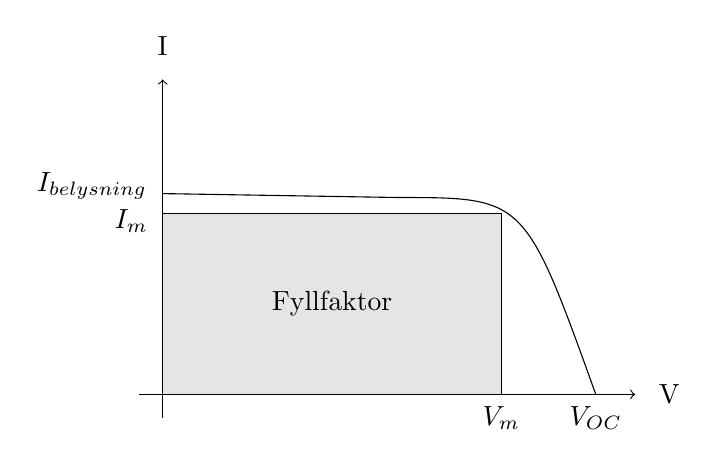
\begin{tikzpicture}

	\draw [->] (-0.3,0) -- (6,0) node [right=5pt]	{V};  % X-akse
	\draw [->] (0,-0.3) -- (0,4) node [above=5pt]	{I}; % Y-akse

	% Faktisk kurve
	\draw [-] (0,2.55) -- (3,2.5);
	\draw [-] (3,2.5) .. controls +(right:1.6cm) .. (5.5,0);
	
	% Fyllfaktor
	\node [draw, rectangle,fill=black!10,minimum height=2.3cm, minimum width=4.3cm] (FF) at (2.15,1.15) {Fyllfaktor};
	
	% Tekst
	\node at (-0.9,2.65) {$I_{belysning}$};
	\node at (-0.4,2.2) {$I_m$};
	\node at (4.3,-0.3) {$V_m$};
	\node at (5.5,-0.3) {$V_{OC}$};
	
	
\end{tikzpicture}

\caption{Str�m-spenningskarakterisitikk med fyllfaktor}%
\label{fig:fyllfaktor}%
\end{figure}

Virkningsgraden til en solcelle er representert ved $\eta$, som er gitt ved:

\begin{equation}
\eta=\frac{P_m}{P_{inn}}=FF \frac{I_{belysning} V_{OC}}{P_{inn}}
\label{eq:virkningsgrad}
\end{equation}

For multikrystallinsk silisium er den h�yeste virkningsgraden som er oppn�dd 18,9 \%. Dette ble oppn�dd av Mitsubishi 28. februar 2009 (fra pressemelding).
\section{Tap}

Mye tap er relatert til s�kalte d�rlige omr�der, hvor det er mye rekombinasjon. Ved � karakterisere d�rlige omr�der, er det mulig � utbedre feil som det finnes kjente metoder for � unng�.

Fotoluminisensspekteret ved romtempratur er dominert av emisjon ved $h\nu_maks=1.09eV$, og et omr�de rundt $0.8eV$.  ~\cite{\tarasov00}

Et eksempel p� dette er fjerning av forurensinger som jern (?) CITATION NEEDED

\subsection{Dislokasjonslinjer}

Dislokasjonslinjer er linjer som kan ses p� spektrometri spekter av eksitert lys fra pr�ven

% dislokasjonsfigur

Det er fire linjer, D1, D2, D3 og D4 som hver har sin s�regne karakteristikk.

\begin{figure}[htbp]
	\centering
		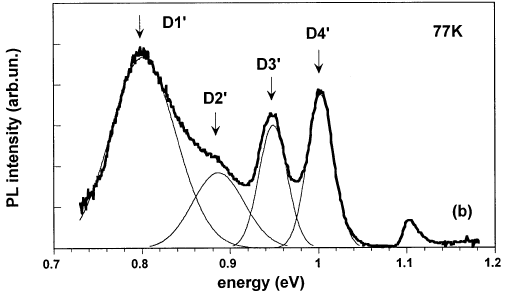
\includegraphics{bilder/dislokasjonslinjer_tarasov00.PNG}
	\label{fig:dislokasjonslinjer}
\end{figure}


Figur \ref{fig:dislokasjonslinjer} viser dislokasjonslinjer for multikrystallinsk silisium ved 77K. D1' er ved 0.80eV, D2' ved 0.89eV, D3' ved 0.95eV og D4' ved 1.00eV \cite{tarasov00}

D1/D2 and D3/D4 belongs to different entities, based on the pl mapping.
\clearpage
\section{M�lemetode og Instrumentering}

En av utfordningene er � f� til et laboppsett som kan m�le og karakterisere ulike former for tap, slik som dislokasjonslinjer, forurensninger, og korngrenser. Dette er viktig for � kunne forst� �rsakene til tap, og for � kunne analysere hvilke framstillingsprosesser som gir et gunstig resultat.

\begin{figure}[H]%
\centering
	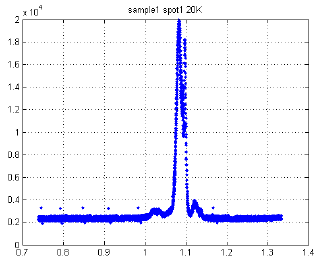
\includegraphics[width=10cm,bb=0 0 332 274]{bilder/cryolabtap.png}%
	\caption{Fotoluminisensspekter ved 20K i cryolab}%
	\label{fig:cryolabtap}%
\end{figure}

Publikasjoner som~\cite{tarasov00} (figur \ref{fig:dislokasjonslinjer}) viser et tapsspekter rundt 0,7-1 eV som ikke er synlig p� m�linger gjort p� cryolab. (figur \ref{fig:cryolabtap}) Grunnen til det er ikke kjent, men antas og v�re et resultat av tap i utstyr som linser og beamsplittere. 1eV tilsvarer 1240nm b�lgelengde fra ~\ref{eq:lysenergi}, som betyr at spekteret som antas � forsvinne har b�lgelengde 1100-1700nm.

\subsection{Laboppsett}
% laboppsett figur her

Eksitert lys fra pr�ven i figur \ref{fig:cryolabtap} g�r gjennom f�lgende komponenter:

\begin{table}[H]
\centering
\begin{tabular}{|c|c|c|c|}
\hline
1 & Vindu p� cryostaten & &  \\
\hline
2 & Objektiv & NT46-405 & \cite{Objektiv} \\
\hline
3 & Beam splitter & BS017 & \cite{beamsplitter} \\
\hline
4 & Linse & ACN127-020-B & \cite{old_lens} \\
\hline
5 & Linse & ACN127-020-B & \cite{old_lens} \\
\hline
6 & Linse & ACN127-020-B & \cite{old_lens} \\
\hline
7 & Spektrometer & iHR550 Imaging Spectrometer & \cite{spektrometer} \\
\hline
8 & Kamera & InGaAs Spectroscopy CCD & \cite{kamera} \\
\hline
\end{tabular}
\caption{Eksisterende lab oppsett p� cryolab}
\label{t:laboppsett1}
\end{table}


Det antas at det er flere kilder til tap blant komponentene som lyset skal gjennom f�r det n�r kameraet. Hoveddelen av tap kommer av refleksjoner, da de optiske komponentene ikke har vesentlig absorbsjon av lyset. Kameraet er oppgitt til � kunne h�ndtere 900 til 1700nm.

Den f�rste komponenten lyset skal gjennom er vinduet i kryostaten, det er oppgitt til � slippe gjennom over 90\% av lyset for b�lgelengder mellom 200nm og nesten helt opp til 2000nm. (Se figur \ref{fig:cryovindu} under vedlegg) Objektivet har en transmisjonfaktor p� rundt 60\% for b�lgelengder mellom 500 og 1800nm. Beamsplitteren er oppgitt til � dele str�len 50:50, med mindre enn 1\% refleksjon (tap) for b�lgelengdene 400-700nm. Men ut ifra figur \ref{fig:beamsplitter400-700nm} er det eksponensielt �kende for b�lgelengder over 700nm. I tillegg forsvinner 50\% av lyset i selve split prosessen. Linsene er oppgitt til � ha under 1\% refleksjon for b�lgelengder mellom 650nm og 1050nm, mens for b�lgelengder utenfor er det eksponensielt �kende refleksjon. Spektrometeret er oppgitt til � ha spektralt spekter fra 150 til 1500nm. 

Dette viser tydelig at beamsplitteren og linsene som er brukt i oppsettet er store kilder til tap, og b�r byttes ut for m�linger med b�lgelengder over 700nm.

\subsection{Forslag til nytt oppsett}

%Hvordan l�se problemet?

Det er tydelig at objektivet, beamsplitteren og linsene er kilder til store tap i systemet. For � kunne gj�re m�linger mellom 1\micro m og 1,5\micro m b�r disse byttes ut med komponenter som har begrenset med tap for de b�lgelengdene som er interessante. For � f� til et st�rre b�lgelengdeomr�de foresl�s det � sette opp en parallell veibane for b�lgelengder fra 1000nm og opp til 1500nm. Dette kan realiseres ved � sette opp speil i str�lebanen som manuelt kan flippes opp og ned for � kontrollere hvor lyset beveger seg.

Forslag til oppsett for parallell optisk vei:

% tegning av parallell veibane

Utstyr for � realisere dette oppsettet kommer fra \url{http://www.thorlabs.de}. F�lgende komponenter er valgt ut:

\begin{table}[H]%
\centering
\begin{tabular}{|c|c|c|}
\hline
Linse & LB4330 & \cite{new_lens} \\
\hline
Speil & PF10-03-P01-10 & \cite{speil} \\
\hline
Iris & ID12SS/M & \cite{iris} \\
\hline
Flip mount (for speil) & FM90/M & \cite{flipmount} \\
\hline
Beam Splitter & BS018 & \cite{beamsplitter_ny} \\
\hline
Post (bordskrue) & TR75/M & \cite{post} \\
\hline
Post holder & PH2/M & \cite{postholder} \\
\hline
Flip mount (for linse) & TRF90/M & \cite{flipmount_linse} \\
\hline
\end{tabular}
\caption{Utstyr til parallell lysbane}
\label{t:nytt_utstyr}
\end{table}

Linsa som er valgt ut skal i f�lge datablad klare over 90\% transmisjon helt opp til 2\micro m i motsetning til det forrige oppsettet. Da m�lingene som skal gj�res kan gj�res over et relativt stort omr�de p� pr�ven er det ikke s� farlig om det belyste omr�det ikke holder 100\% fokus, slik at et avvik p� noen grader i str�lebanen ikke er kritisk for resultatet. Det kun trengs en linse p� den parallelle banen for � fokusere inn til spektrometeret som alene gj�r at det blir mindre tap. Beamsplitteren er oppgitt til � ha mindre enn 0.3\% refleksjon for b�lgelengdene 1.1 til 1.6\micro m. Det vil fortsatt forvinne 50\% intensitet her p� grunn av at lyset splittes, men det frekvensavhengige tapet er i f�lge datablad mye mindre for disse b�lgelengdene. % legge til appendix / referere til figurer?

% laser b�lgelengde? for h�y intensitet til at tapet har s� mye � si?

Speil monteres p� en s�kalt 'flip mount', slik at det kan skrus fast i det optiske bordet i en bestemt posisjon, og vippes 90 grader inn eller ut av str�lebanen, slik at det blir en parallell optisk bane for lyset � f�lge n�r m�linger som antas � ligge over 1000nm skal gj�res.

%linser her ogs�?

% figur.

For � teste det nye lapoppsettet, er det tatt i bruk en pr�ve med Erbium som er gitt at skal lyse opp rundt 1550 (se fig. \ref{fig:erbium_eksitasjon}). Denne pr�ven har et absorbsjonsspekter som vist i figur \ref{fig:erbium_absorbsjon} som gj�r gr�nn laser p� 532nm s�rdeles godt egnet som pumpelys.

% Er absorbsjon figur

% Er eksitasjonfigur
%\begin{figure}[!h]
\centering
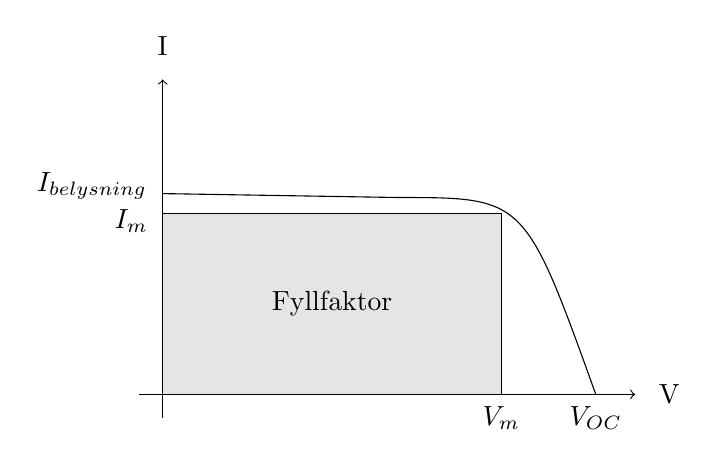
\begin{tikzpicture}

	\draw [->] (-0.3,0) -- (6,0) node [right=5pt]	{V};  % X-akse
	\draw [->] (0,-0.3) -- (0,4) node [above=5pt]	{I}; % Y-akse

	% Faktisk kurve
	\draw [-] (0,2.55) -- (3,2.5);
	\draw [-] (3,2.5) .. controls +(right:1.6cm) .. (5.5,0);
	
	% Fyllfaktor
	\node [draw, rectangle,fill=black!10,minimum height=2.3cm, minimum width=4.3cm] (FF) at (2.15,1.15) {Fyllfaktor};
	
	% Tekst
	\node at (-0.9,2.65) {$I_{belysning}$};
	\node at (-0.4,2.2) {$I_m$};
	\node at (4.3,-0.3) {$V_m$};
	\node at (5.5,-0.3) {$V_{OC}$};
	
	
\end{tikzpicture}

\caption{Str�m-spenningskarakterisitikken for en solcelle}%
\label{fig:fyllfaktor}%
\end{figure}

\clearpage
\appendix
\section{Transmisjonskurver}

\begin{figure}[H]%
\centering
%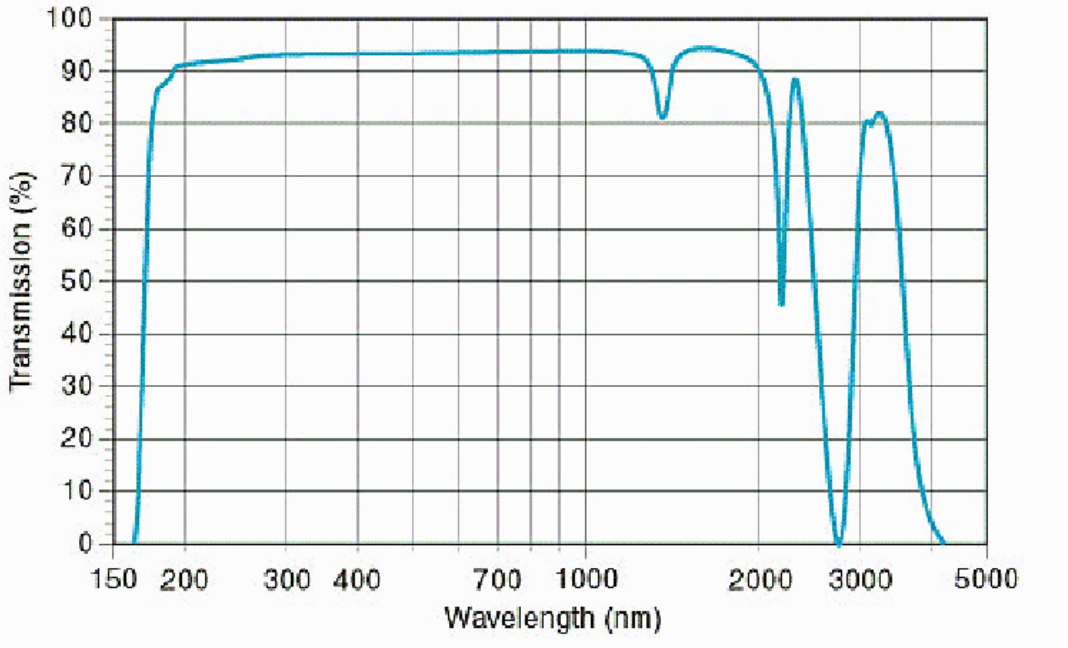
\includegraphics[width=10cm,bb=0 0 1068 648]{cryovindu}%
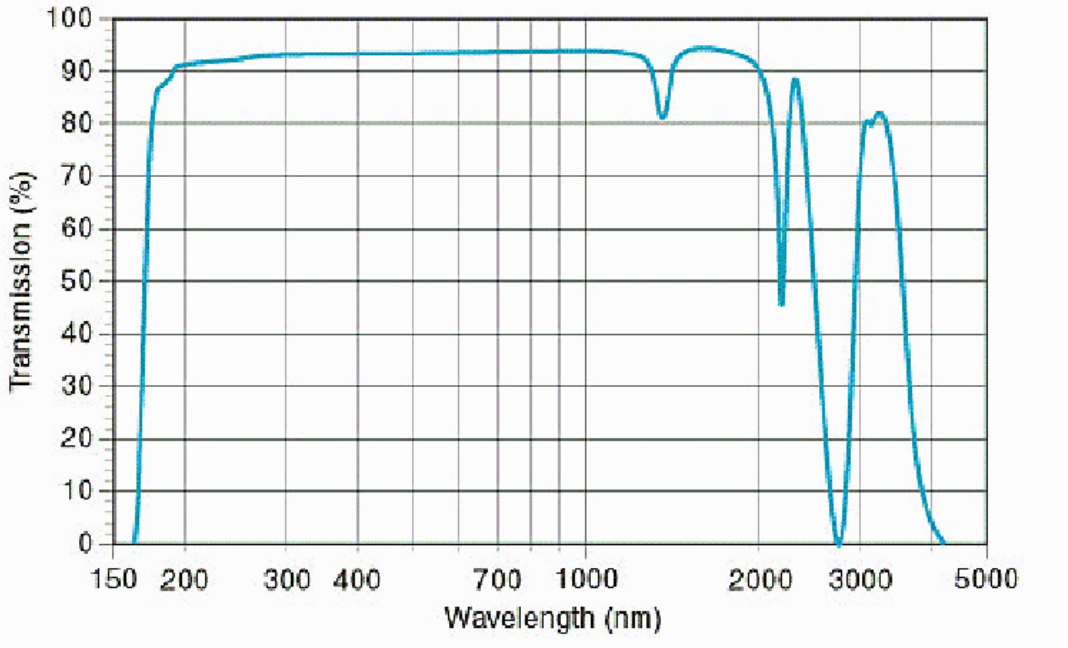
\includegraphics[width=10cm]{cryovindu}%
\caption{Transmisjon gjennom viduet til cryostaten \cite{cryostat} 27.10.2009}%
\label{fig:cryovindu}%
\end{figure}

\begin{figure}[H]%
\centering
%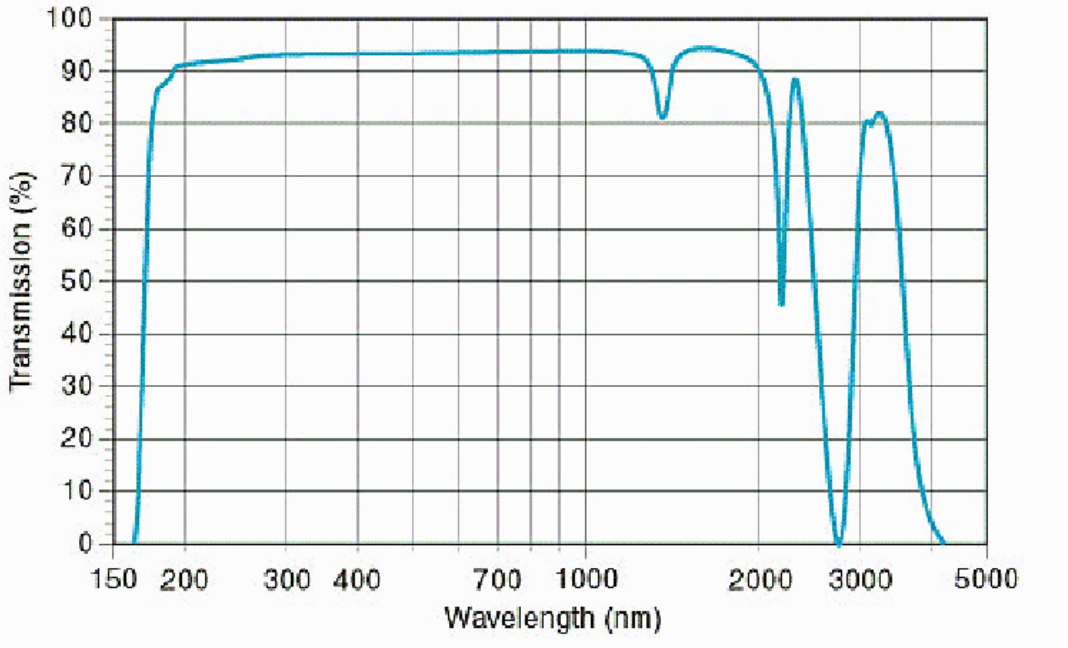
\includegraphics[width=10cm,bb=0 0 1068 648]{cryovindu}%
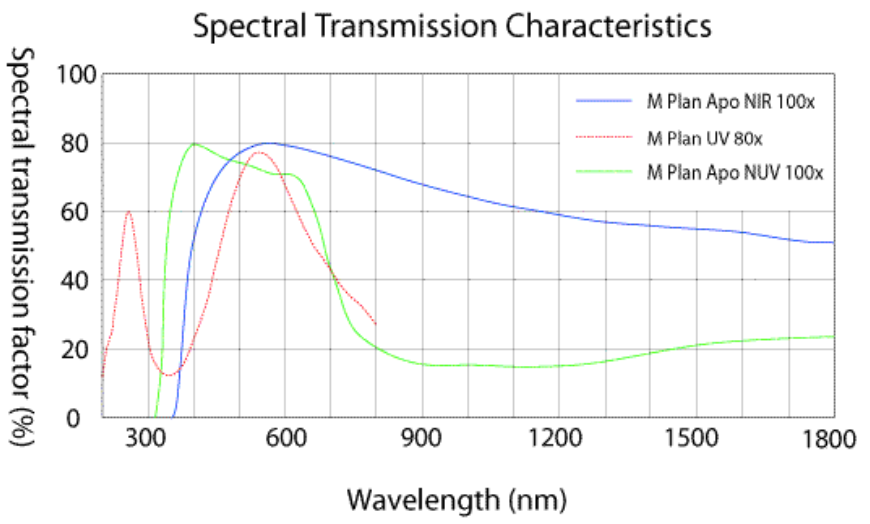
\includegraphics[width=10cm]{objektiv}%
\caption{Transmisjon gjennom objektivet \cite{objektiv} 08.12.2009}%
\label{fig:objektiv}%
\end{figure}

\begin{figure}[H]%
\centering
%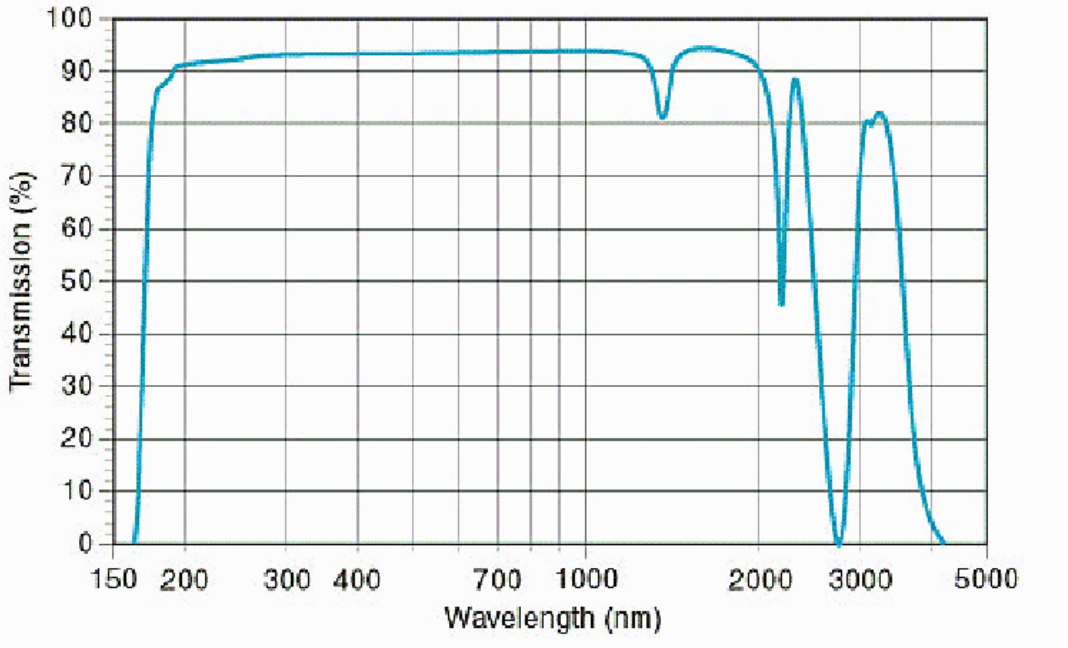
\includegraphics[width=10cm,bb=0 0 1068 648]{cryovindu}%
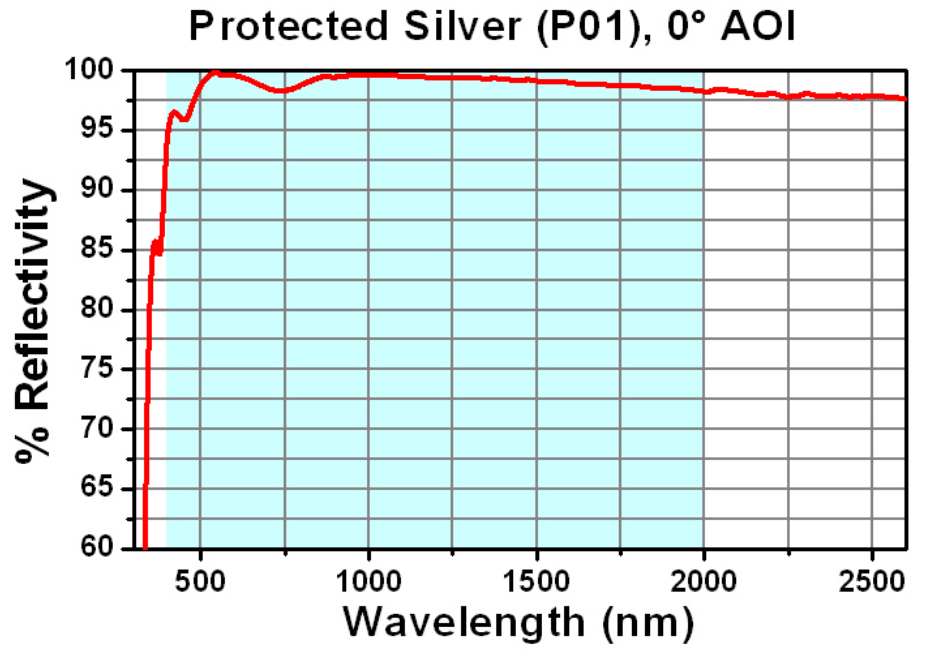
\includegraphics[width=10cm]{speil}%
\caption{Refleksjon for speil \cite{speil} 08.12.2009}%
\label{fig:speil}%
\end{figure}

\begin{figure}[H]%
\centering
%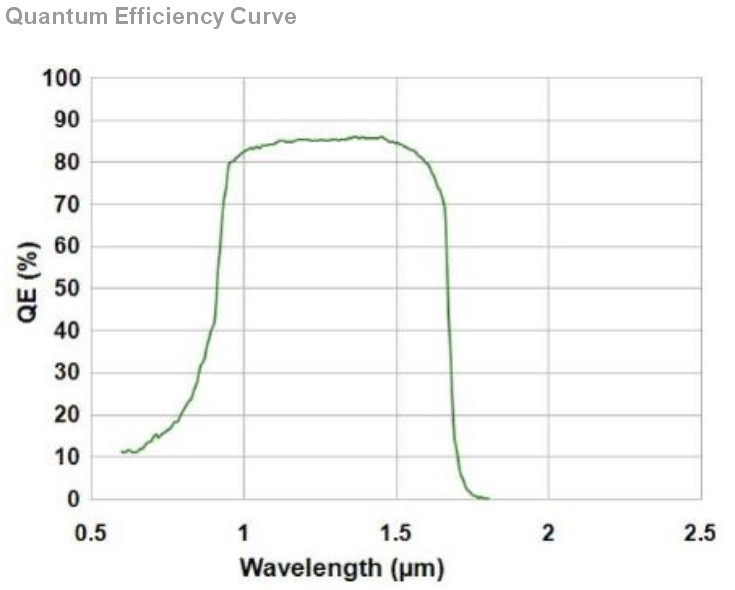
\includegraphics[width=10cm,bb=0 0 735 590]{kameragraf}%
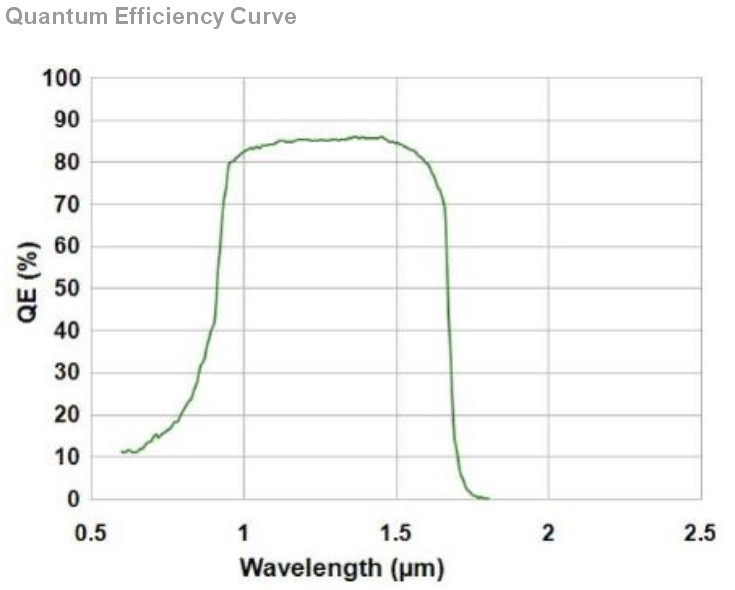
\includegraphics[width=10cm]{kameragraf}%
\caption{Kameraeffektivitet \cite{kamera} 27.10.2009}%
\label{fig:kameragraf}%
\end{figure}



\subsection{F�rste veibane}

\begin{figure}[H]%
\centering
%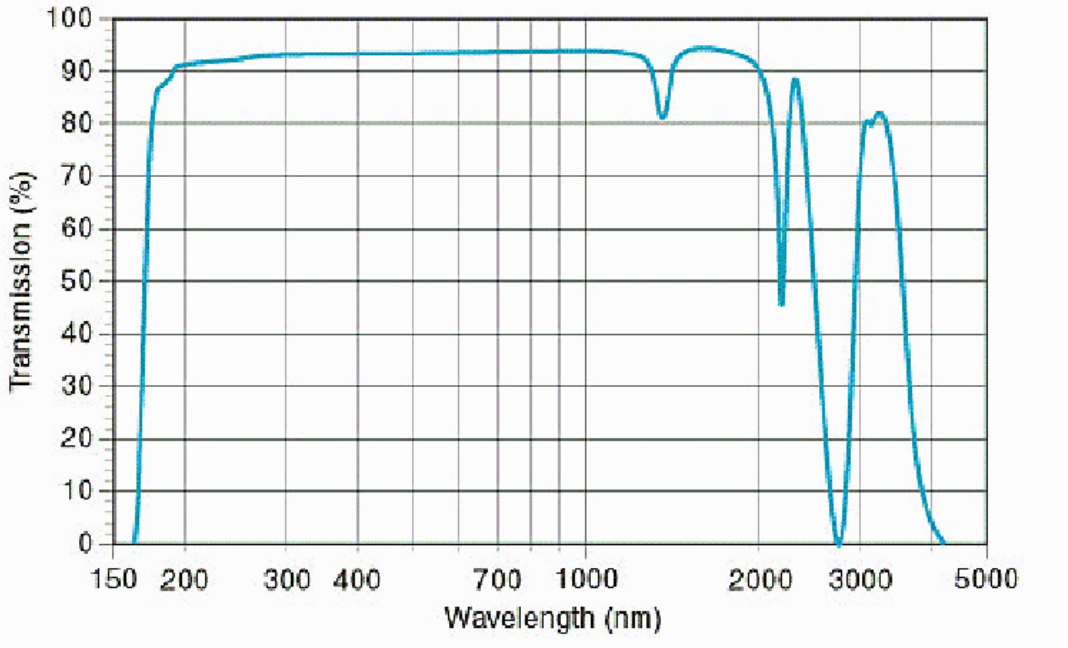
\includegraphics[width=10cm,bb=0 0 1068 648]{cryovindu}%
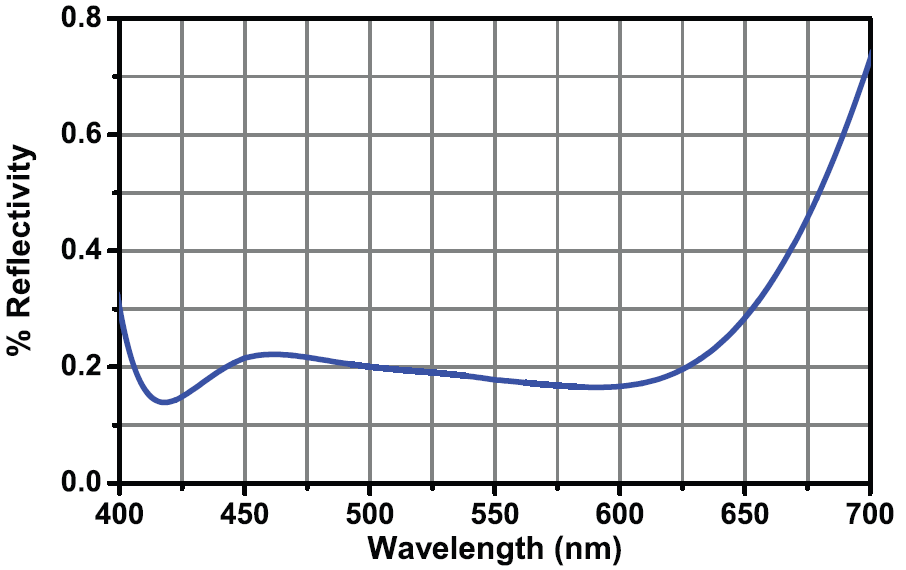
\includegraphics[width=10cm]{breamsplitter400-700nm}%
\caption[Beamsplitter 400-700nm]{Beamsplitter refleksjon fra datablad optimalisert for 400-700nm \cite{beamsplitter} 12.12.2009}%
\label{fig:beamsplitter400-700nm}%
\end{figure}

\begin{figure}[H]%
\centering
%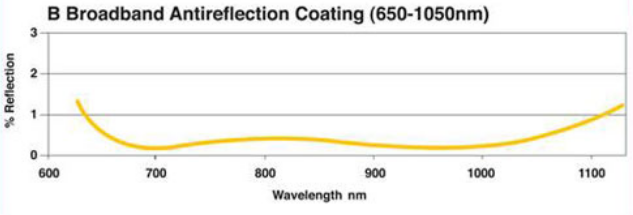
\includegraphics[width=10cm,bb=0 0 633 215]{old_linse}%
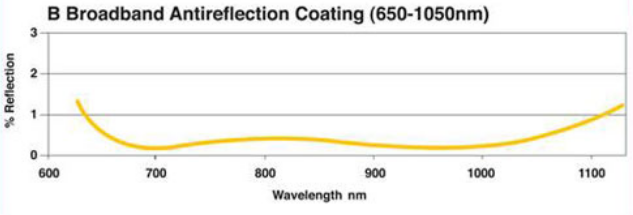
\includegraphics[width=\columnwidth]{old_linse}%
\caption{Transmisjon gjennom linse fra gammel veibane \cite{old_lens} 27.10.2009}%
\label{fig:linsetrans}%
\end{figure}

\subsection{Andre veibane}

\begin{figure}[H]%
\centering
%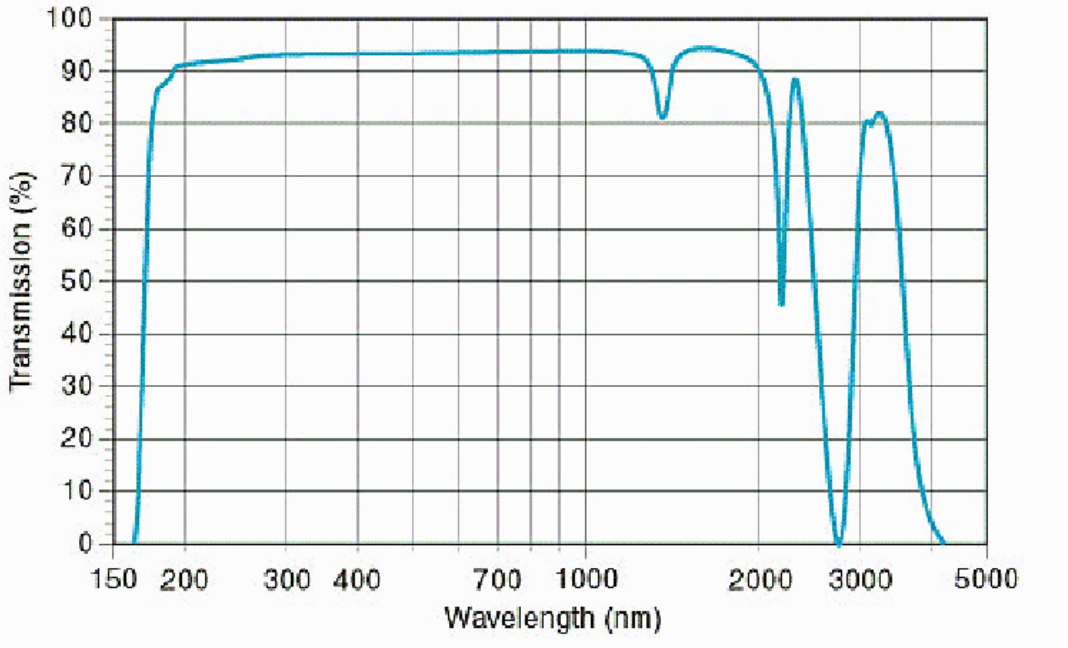
\includegraphics[width=10cm,bb=0 0 1068 648]{cryovindu}%
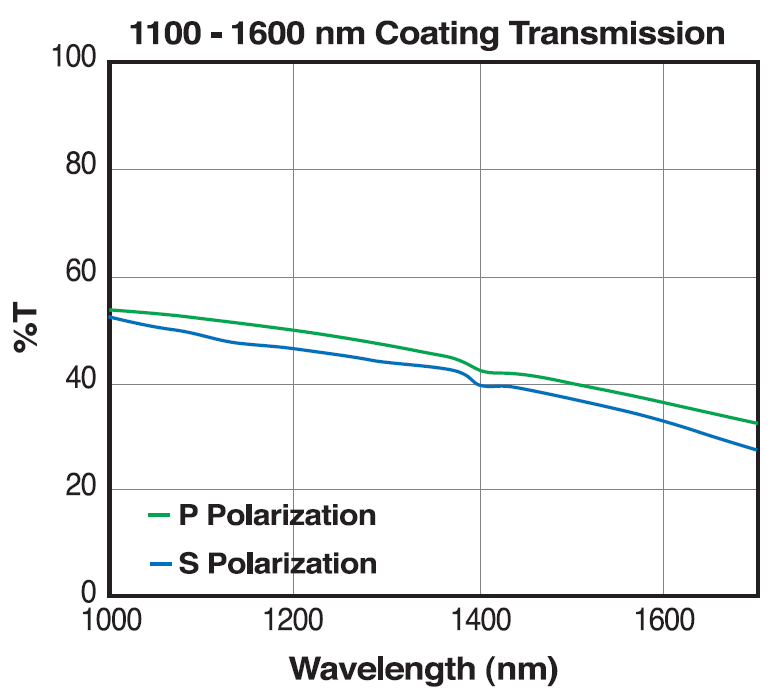
\includegraphics[width=10cm]{breamsplitter1100-1600nm}%
\caption[Beamsplitter 1100-1600nm]{Beamsplitter refleksjon fra datablad optimalisert for 1100-1600nm \cite{beamsplitter_ny} 12.12.2009}%
\label{fig:beamsplitter1100-1600nm}%
\end{figure}

\begin{figure}[H]%
\centering
%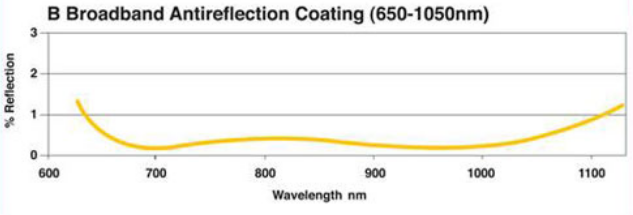
\includegraphics[width=10cm,bb=0 0 633 215]{old_linse}%
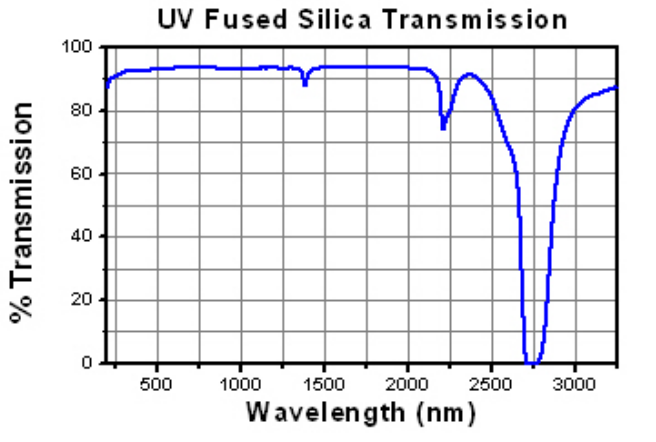
\includegraphics[width=10cm]{ny_linse}%
\caption{Transmisjon gjennom ny linse \cite{new_lens} 08.12.2009}%
\label{fig:linsetrans_ny}%
\end{figure}

\clearpage
\bibliographystyle{plain}
\nocite{}

\bibliography{bibliography} % bibliography.bib


\end{document}

% Referanseliste

